

In this section, I present some background knowledge that builds a foundation for the rest of the dissertation. I start by describing the theme of this dissertation: Affective Computing, a fast-growing branch in Computer Science. As one of the hottest topics in Affective Computing, mental disorder detection is discussed. I detail the audio-visual feature extraction commonly used in the area of Affective Computing and the basics in multi-modality are present along with the potential in automatic detection of Bipolar Disorder.










\section{Affective Computing}

Traditional Human-Computer Interaction (HCI) designs usually involves interface devices such as keyboards or touch-screens, which emphasize the transmission of explicit messages, while completely ignoring implicit information of users, like users' affective states \cite{zeng2008}. This limitation makes the interaction cold, incompetent, and socially inept, and a shift from computer-centered interfaces to human-centered interfaces is called for \cite{pantic2007}. As a fundamental component of human-human communication, users' affective states has gradually become a new focus for HCI \cite{cohn2007} and specifically, affect-sensitive HCI systems must be capable of detecting and understanding subtleties of users' affective behaviour before responding to users' commands. For Affective Computing, the recognition and modelling problems have been simplified by the assumption of a small set of discrete emotions, or a small number of dimensions \cite{picard2000}, such as Arousal-Valence dimension space \cite{barrett1998}, as shown in Figure \ref{fig:arousal_valence}.

\begin{figure}
    \centering
    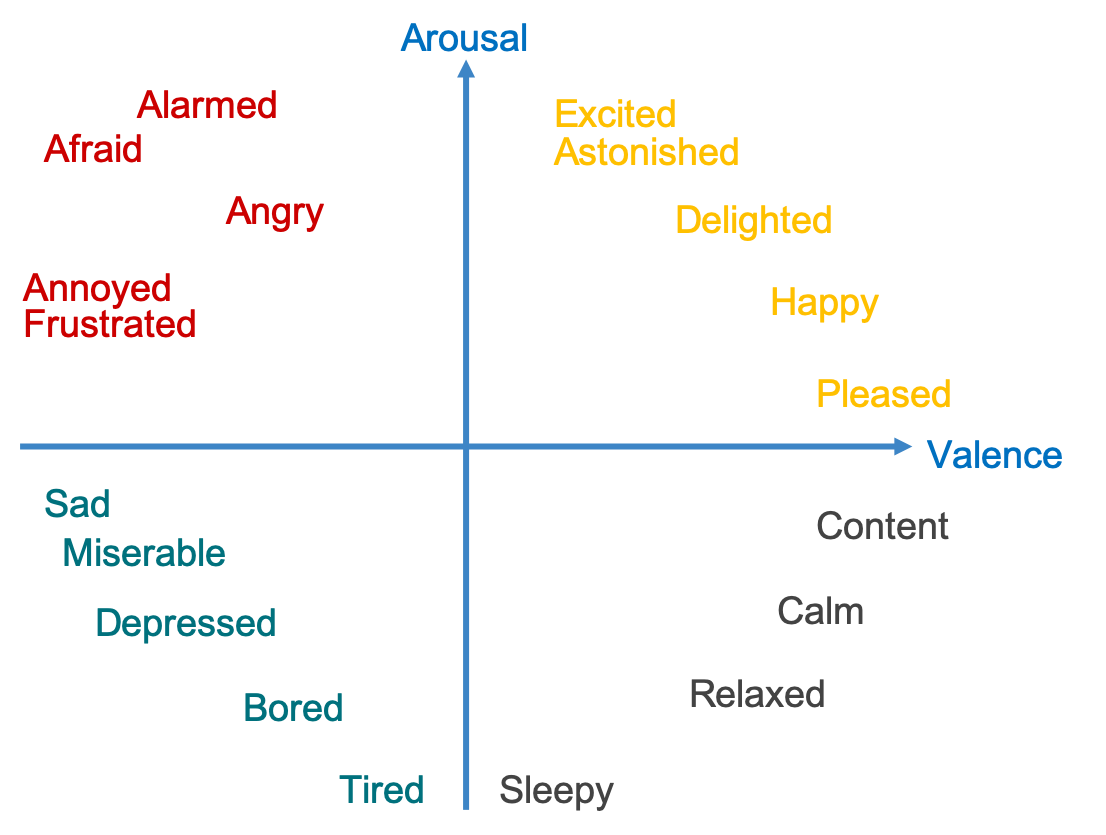
\includegraphics[width=10cm]{images/background/arousal_valence.png}
    \caption{Arousal-Valence dimension space with exemplar emotions}
    \label{fig:arousal_valence}
\end{figure}


Affective Computing is an interdisciplinary field that focuses on the study and development of systems that can recognize, interpret, process and express human affects. It spans Computer Science, Psychology, and Cognitive Science. Affect-sensitive interfaces are being developed in a number of domains to automatically recognizing and responding to users' affective states, including gaming, mental health, and learning technologies \cite{calvo2010}. For instance, an affect-sensitive tutoring system, called AutoTutor, could simulate human tutors and improve students' learning gains by detecting their emotional responses, like frustration \cite{sidney2005}.









\section{Mental Disorder Detection}

With the advancement in the field of Affective Computing, a large set of affective issues have been tackled, ranging from short-term states (e.g. laughter, emotions), to mid-term disorders (e.g. depression, bipolar disorder, or autism) and to long-term traits (e.g. personality traits) \cite{picard2000, schuller2011}. 

While the discrete emotions could be detected in shorter frames, the recognition of mid-term disorders needs to detect distinct emotions to indicate disorders as healthcare professionals do, and also take into account of temporal information \cite{picard2000, yacoob1994, zacharatos2014}. Temporal descriptors for both acoustic and visual modalities have been shown to provide more information for mental disorder detection \cite{ambadar2005, joshi2013}. Within the past several years, various models have been investigated for depression level estimation from behavioural observations \cite{cohn2007, cummins2011}, such as Gaussian Mixture Models (GMM), Support Vector Machines, Relevance Vector Regression (PVR), and even Deep Neural Networks (DNN). These proposed models proved promising results in some challenges, and for example, GMMs achieved an F1 mean score 0.81 in a binary depression detection compared with 0.73 in the baseline system \cite{williamson2016}. The automated approach for depression evaluation can be transferred to the detection of other mental disorders, such as bipolar disorder (BD).




\section{Audio-Visual Feature Extraction}

Arguably, the most important step in the automatic recognition of BD or other emotion-related tasks is the extraction of audio-visual features that must be relevant and provide a compact representation of each sample \cite{schuller2011}. The following subsections will discuss three commonly used audio-visual features in Affective Computing.



\subsection{MFCC}

In speech processing, Mel-Frequency Cepstrum Coefficients (MFCCs) have been the dominant features because of their ability to represent the speech amplitude spectrum in a compact form \cite{young1993htk}. Figure \ref{fig:mfcc_procedure} shows the procedure of the generation of MFCC features. The first step is to divide the audio signal into frames with equal length, usually by applying a window function, typically a Hamming window. The window function removes edge effects or noise in the background. A cepstral feature vector is then generated for each frame and Discrete Fourier Transform is applied on the vector. In the next step, only the logarithm of the amplitude spectrum is retained as amplitude is proven more important than phase information. Before taking a discrete cosine transform, the vector is Mel-scaled and smoothed first to emphasize perceptually meaningful frequencies. The Mel-scale relates perceived frequency, or pitch, of a pure tone to its measured frequency. The formula for converting from frequency to Mel scale is as follows.

\begin{equation}
    M(f) = 1125 \ln(1+f/700)
\end{equation}


\begin{figure}[htb]
    \centering
    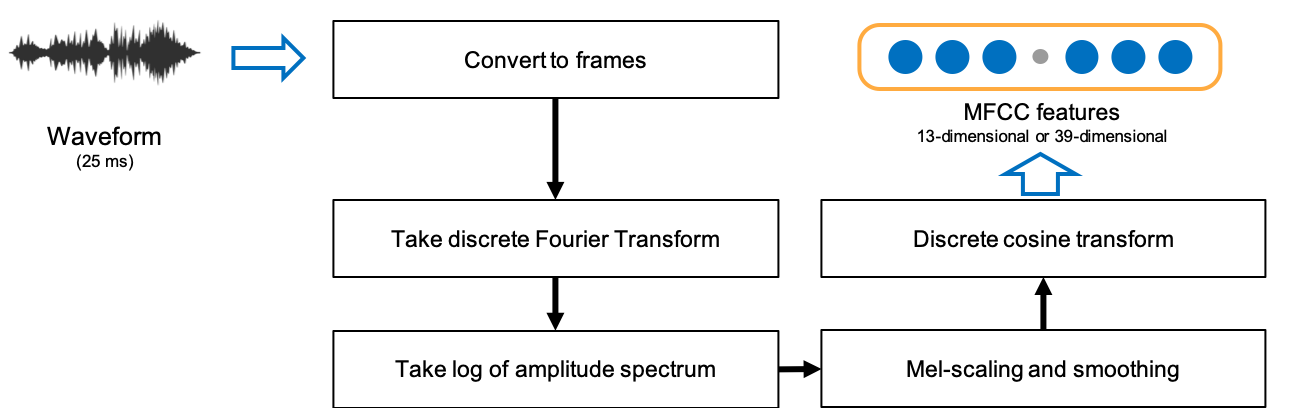
\includegraphics[width=12cm]{images/background/mfcc_procedure.png}
    \caption{MFCC features generation procedure}
    \label{fig:mfcc_procedure}
\end{figure}

The components in resulting Mel-spectral vectors for each frame are highly correlated and then Discrete Cosine Transform is used to decorrelate these components, generating 13 cepstral features on frame level. Generally, MFCCs from 25ms audio frames (sampled at a rate of 10ms) have dimensionality 13 from 26 Mel-Frequency bands. Additional 13 delta ($1^{st}$-order derivative) and 13 acceleration ($2^{nd}$-order derivative) coefficients could be appended to the MFCCs with a cepstral filter with a weight parameter of 22. MFCCs are commonly used as low-level descriptors (LLDs) in many audio signal processing tasks.




\subsection{GeMAPS and eGeMAPS}

Much of recent research considers the extraction of acoustic features as a method to understand the patterning of the vocal expression of different emotions \cite{juslin2001, yildirim2004, eyben2015}. The underlying theoretical assumption is that the affective processes influence autonomic arousal and the tension of the striated musculature at different scales and thus affect voice and speech production \cite{scherer1986}. These emotion-differentiating changes, if measured and extracted as a compact parameter set, could probably improve the performance recognition systems in BD.

Following this principle, Eyben \textit{et al.} proposed GeMAPS (and eGeMAPS) as a standard acoustic parameter set for voice analysis. GeMAPS stands for the Geneva Minimalistic Acoustic Parameter Set and it is a basic standard acoustic parameter set for various areas of automatic voice analysis. These parameters are selected based on the potential to index affective physiological changes in voice production, the proven value in former studies as well as the automatic extractability, and the theoretical significance. eGeMAPS, on the other hand, is the extended version of GeMAPS with additional cepstral parameters, and the full list refers to Table \ref{tab:list_egemaps}.

\begin{table}[ht]
    \small
    \centering
    \caption{Complete list of GeMAPS and eGeMAPS (parameters \textbf{in bold} are additional parameters only in eGeMAPS)}
    \begin{tabular}{p{3.5cm}|p{9cm}}
        \Xhline{2\arrayrulewidth}
        Parameter Name & Description \\
        \hline
        \multicolumn{2}{l}{Frequency Related Parameters} \\
        \hline
        Pitch & Logarithmic fundamental frequency $F_0$ on a semitone frequency scale \\
        Jitter & Deviations in individual consecutive $F_0$ period lengths \\
        Formant 1, 2, and 3 frequency & Centre frequency of 1st, 2nd, and 3rd formant \\
        Formant 1 & Bandwidth of 1st formant \\
        \textbf{Formant 2-3} & Bandwidth added for completeness \\
        \hline
        \multicolumn{2}{l}{Amplitude Related Parameters} \\
        \hline
        Shimmer & Difference of the peak amplitudes of consecutive $F_0$ periods \\
        Loudness & Estimate of perceived signal intensity from an auditory spectrum \\
        Harmonics-to-Noise Ratio & Relation of energy in harmonic components to energy in noise-like components \\
        \hline
        \multicolumn{2}{l}{Spectral Related Parameters} \\
        \hline
        Alpha Ratio & Ratio of the summed energy from 50-1000 Hz and 1-5 kHz \\
        Hammarberg Index & Ratio of the strongest energy peak in region 0-2kHz to the strongest peak in region 2-5 kHz \\
        Spectral Slop & Linear regression slope of the logarithmic power spectrum within 0-500 Hz and 500-1500 Hz \\
        Formant 1, 2, and 3 relative energy & Ratio of the energy of the spectral harmonic peak at 1st, 2nd, 3rd formant's centre frequency to the energy of the spectral peak at $F_0$ \\
        Harmonic difference H1-H2 & Ratio of energy of the first $F_0$ harmonic (H1) to the energy of the second $F_0$ harmonic (H2) \\
        Harmonic difference H1-A3 & Ratio of energy of the first $F_0$ (H1) to the energy of the highest harmonic in the third formant range (A3) \\
        \textbf{MFCC 1-4} & Mel-Frequency Cepstral Coefficients 1-4 \\
        \textbf{Spectral flux} & Difference of the spectra of two consecutive frames \\
        \Xhline{2\arrayrulewidth}
    \end{tabular}
    \label{tab:list_egemaps}
\end{table}





\subsection{Facial Action Units}

Facial behaviour can be defined as \textit{facial landmarks}, \textit{head pose}, \textit{eye gaze}, and \textit{facial expressions}, each of which plays an important role individually and collectively \cite{baltrusaitis2018}. Facial landmarks allow us to understand facial expression motion and the dynamics along with the benefits for face alignments in various tasks such as gender detection and age estimation \cite{fu2010age}. Head pose has been demonstrated its usefulness in emotion recognition and social signal perception \cite{adams2015}, and eye gaze has also been proved effective when evaluating attentiveness, social skills, mental health \cite{vail2017}, and intensity of emotions \cite{kleinke1986}. Facial expression, usually represented by Facial Action Units (FAUs), is both powerful and natural mean of inter-personal communication and emotions can be interpreted as a complex combination of several facial expressions \cite{ekman2013}. To detect and measure a large number of facial expressions, Ekman and Friesen \cite{ekman1976} developed the Facial Action Coding System (FACS), which is widely used for facial behaviour analysis to date. Their approach was, however, expensive and time-consuming as the selection of AUs was based on a small set of muscular actions observed and manually scored by the trained experts \cite{ekman1976}. Therefore, for automatic facial behaviour analysis and understanding, a system capable of recognizing \textit{facial landmarks}, \textit{head pose}, \textit{eye gaze}, and \textit{FAUs} without human intervention has been an active research topic.


\begin{figure}[ht]
    \centering
    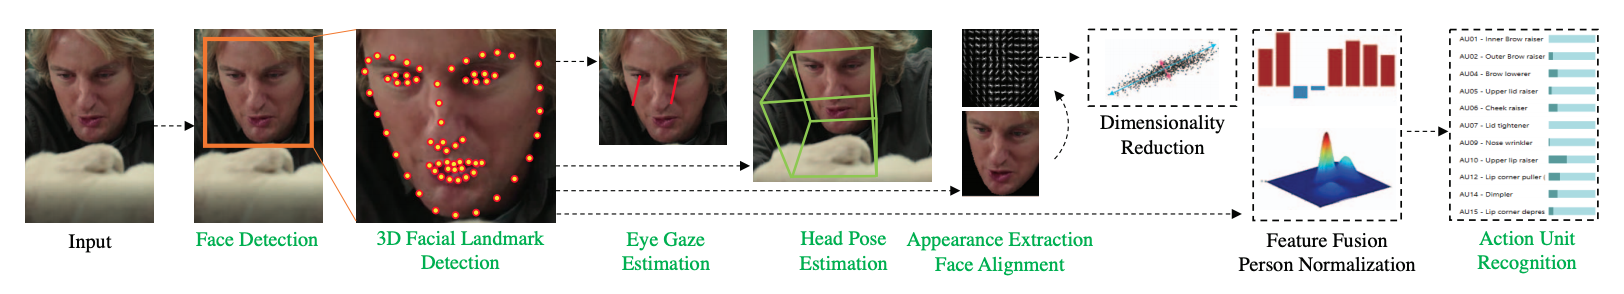
\includegraphics[width=1.1\textwidth]{images/background/openface.png}
    \caption[OpenFace 2.0 facial behaviour extraction pipeline]{OpenFace 2.0 facial behaviour extraction pipeline (taken from \cite{baltrusaitis2018})}
    \label{fig:openface}
\end{figure}


OpenFace 2.0, proposed by Baltrusaitis \textit{et al.} \cite{baltrusaitis2018} was an automatic toolkit on real-time data for facial landmark detection, head pose estimation, eye gaze determination, and facial action units recognition. The general pipeline of OpenFace 2.0 refers to Figure \ref{fig:openface}. OpenFace 2.0 was demonstrated state-of-the-art results in their experiment \cite{baltrusaitis2018}, and was used as the baseline extractor for visual features in many studies in Affective Computing communities. 



\section{Multimodal Learning}

Intuitively speaking, we interact with the surrounding world in different ways - we see objects, we hear sounds and we smell odours - and in other words, the world involves multiple modalities. A modality refers to a particular mode in which something happens or is experienced. When a research problem or dataset includes multiple modalities, it can be therefore characterized as multimodal. 


Multimodal learning is intended to build models that can process and relate information from multiple modalities \cite{baltruvsaitis2017}. Multimodal learning has been introduced with the motivation of the McGurk effect \cite{mcgurk1976} in Audio-Visual Speech Recognition (AVSR) that the visual input has been demonstrated influential in speech perception. In the following research, the experimental results showed that supplementary modalities, such as visual information in AVSR, improve the robustness of the multimodal models \cite{gurban2008} and the performance of the model in noisy scenarios \cite{ngiam2011}. 

In addition to AVSR, multimodal learning has also been applied to the automatic understanding of human multimodal behaviors in social interactions \cite{baltruvsaitis2017}. With the technical advances in face detection, facial landmark localization, and facial expression recognition \cite{kanade2005}, Audio-Visual Emotion Challenge (AVEC) has been introduced in 2011 to further the multimodal information processing and its application in healthcare and emotion recognition \cite{schuller2011}.

In my work, I only concentrate on three modalities, visual signals which are represented with images or video, acoustic signals which encode sounds and para-verbal information, and natural language which is spoken by the interview subjects. 